\documentclass[a4paper,11pt]{book}
\usepackage{natbib}
\usepackage{tabu, longtable}
\usepackage{pdflscape}
\usepackage[table]{xcolor}
\usepackage{tablefootnote}
\usepackage{hyperref}
\usepackage{graphicx}


%MACROS

%footnotes in tables
%\makesavenoteenv{tabular}

% shade rows in table
%\rowcolors{2}{gray!15}{white}

% alternate rowcolors for all tables
\let\oldtabular\tabular
\let\endoldtabular\endtabular
\renewenvironment{tabular}{\rowcolors{2}{white}{gray!15}\oldtabular}{\endoldtabular}

% alternate rowcolors for all long-tables
\let\oldlongtable\longtable
\let\endoldlongtable\endlongtable
\renewenvironment{longtable}{\rowcolors{2}{white}{gray!15}\oldlongtable} {
\endoldlongtable}



% allow column widths in tables with alignment
\newcolumntype{L}[1]{>{\raggedright\let\newline\\\arraybackslash\hspace{0pt}}m{#1}}
\newcolumntype{C}[1]{>{\centering\let\newline\\\arraybackslash\hspace{0pt}}m{#1}}
\newcolumntype{R}[1]{>{\raggedleft\let\newline\\\arraybackslash\hspace{0pt}}m{#1}}


%\chapter{Introduction}
%\section{Generation of Promoter Capture Hi-C interaction maps across 17 primary human cell types}
%\chapter{Methods and Materials}
%	\section{Collection and Quality control of GWAS summary statistics from 31 genome wide association studies}
%	\section{Poor Man's Imputation (PMI) - Imputation of GWAS p-values to 1000 Genome reference with missing direction of effect information}
%	\section{Fine mapping using approximate Bayes factors}
%	\section{blockshifter - A competitive test for associated variant enrichment in PHCiC interactions maps}
%	\section{COGS - An algorithm for PCHiC assisted prioritisation of genes and tissue contexts}
%	\section{COGS gene set enrichment analysis}
%	\section{Measurement of Allelic imbalance in IL2RA}
%\chapter{Results}
%	\section{Comparison of PMI with Genotype level imputation}
%	\section{Tissue specific enrichment of associated variants with PIRs across 31 traits}
%	\section{PCHiC assisted gene prioritisation across 31 traits}
%	\section{Fine mapping and gene prioritisation across 8 densely genotyped autoimmune diseases}
%	\section{Promoter contacts underlie context specific allelic expression of IL2RA}  
%\chapter{Discussion and Future Work}
%	\section{CHiCP - A platform for visual integration and results disemination}
%   \section{blockshifter and COGS refinement}
%   		\subsection{Assumption examination}
%       \subsection{Stand alone code development}
%   		\subsection{Data driven approach to understanding COGS scores}
%   		\subsection{Integration of functional data through data driven variable priors}
%   		\subsection{How prevelent are dual function coding SNPs ?}
%   		\subsection{PCHiC eQTL and GWAS colocalisation} 
%	\section{Development of methods for tissue specific gene set enrichment analysis}
%	\section{PCHiC modeling of local gene networks}
%	\section{Acknowledgements}
%\tableofcontents
%\end{document}

% define the title
\author{Oliver S Burren}
\title{First Year Report}
\begin{document}
% generates the title
\maketitle
% insert the table of contents
\tableofcontents
\chapter{Introduction}
A fundamental challenge in biology is understanding the genetic and molecular basis of Autoimmunity. Genome-wide association studies (GWAS) have identified at least 324 distinct genetic loci associated with one or more autoimmune diseases (http://www.immunobase.org). Focus is now drawn to elucidating the mechanisms by which causal variation modulates phenotypic endpoints, a prerequisite for successful therapeutic development. The majority of associated variants fall outside of genes \cite{MauranoHumbertRynesEtAl2012} and the integrative analysis of chromatin marks with GWAS highlights a tissue specific specific regulatory role \cite{FarhMarsonZhuEtAl2015}.  Recent studies \cite{SmemoTenaKimEtAl2014,Davison2012-zk} have shown that such regulatory variants might, through chromatin conformation, regulate distal genes. However, further progress in this area has been hampered by incomplete knowledge of causal variants and the target genes and the specific tissue contexts in which they operate\cite{Albert2015-jn}. 

Fine mapping is the process of refining association signals in a region in order to characterise fine scale genetic architecture, a neccessary step in order to identify putative causal variants. Progress in this area is challenging, due to the presence of linkage disequillibrium (LD), which in many cases means that the causal variation cannot be resolved statistically.  This has driven the the development of integrative techniques that couple fine mapping methods with functional information to prioritise causal variants, genes and tissue contexts for targetted empirical interrogation. Examples include Bayesian hierachical modelling \cite{Pickrell2014-xs} and the integration of eQTL datasets using mendelian randomisation\cite{ZhuZhangHuEtAl2016}, however to date systematic methods for incorporating physical interactions between variants and their target genes have not been attempted.  

Recently techniques such as Hi-C\cite{Lieberman-AidenvanBerkumWilliamsEtAl2009} and ChIA-PET\cite{FullwoodLiuPanEtAl2009} have been developed to map the genome-wide chromatin interactions in specific cell types\cite{RaoHuntleyDurandEtAl2014}. Promoter capture Hi-C (PCHi-C) incorporates a sequence capture extension to classical Hi-C to enrich for chromatin interactions with protein coding gene promoters. 

In this report I describe the development of a methological framework that can be used to integrate tissue specifc PCHi-C interaction maps with both targeted and genome wide genetic studies. Using a set of interaction maps for 17 haematopoietic primary Human cell types and focussing on autoimmunity I use this framework to define lists of prioritised variants, genes and cellular contexts. I show how these can be further refined by using  deep genomic phenotyping of  CD4$^{+}$ T cells  in activated and non-activated states. Finally I describe followup experiments in \textit{IL2RA} that demonstrate context specific allelic imbalance, that provides validation of this framework.

\chapter{Materials and Methods}
\section{Collection and quality control of GWAS summary statistics from 31 genome wide association studies}
Define here where we got the interaction data from CHiCAGO, and where we obtained the GWAS summary statistics.
\section{Poor Man's Imputation (PMI) - Imputation of GWAS p-values to the 1000 Genome reference panel in the absence of effect size and direction}
We developed a pipeline that approximates the $p$-value for missing SNP summary statistics for a given study using a suitable reference genotype set. Firstly the genome is split into regions based on a recombination frequency of 0.1cM using HapMap recombination rate data. For each region we retrieve from the reference genotype set (1000 genomes EUR cohort) all SNPs that have MAF $ > 1\%$ and use these to compute pairwise LD. We pair each SNP with missing $p$-values to the SNP with maximum pairwise $r^2$, ${r^2}_{max}$, if that ${r^2}_{max} > 0.6$, and impute the missing $p$-value as that at the paired SNP. SNPs with missing data or without a pair above threshold are discarded as are SNPs that are included in the study but don’t map to the reference genotype set. . 
\section{Genetic fine mapping of 31 traits using approximate Bayes factors}
To further increase resolution we use Wakefield’s synthesis of approximate Bayes factors\cite{Wakefield2009b}  to compute posterior probabilities for each SNP\cite{MallerMcVeanEtAl2012} within a 0.1 cM region.

% add equation here with an explanation

\begin{equation}
	P(SNP_{i} causal | Data) = \frac{BF_{i}\pi_{i}}{1 + \sum_{i=1} BF_{i}\pi_{i}}
\end{equation}

We masked the MHC region (GRCh37:chr6:25-35Mb) from all downstream analysis due to its extended LD and known strong and complex association with autoimmune diseases
\section{blockshifter - A competitive test for assocated variant enrichment in PCHiC interaction maps}
We developed a method based on ideas implemented in \textit{GOSHIFTER} to examine the enrichment of GWAS signals in the promoter interacting regions (PIR) in order to overcome linkage disequilibrium (LD) and interaction fragment correlation. \textit{blockshifter}  implements a competitive test of enrichment between a test set of PIRs compared to a control set. Firstly the coordinates of the PIRs in the union of test and control sets are retrieved, and PIRs with no GWAS signal overlap, or that are found in both test or control set are discarded. For the remaining PIRs we store the number and sum of overlapping GWAS posterior probabilities and these are used to compute $\delta$, the difference in the means between the test and control set . Due to correlation between GWAS signals and between PIRs the variance of $\delta$ is inflated we thus compute it empirically using permutation.  Runs of one or more PIRs (separated by at most one \textit{Hind}III fragment) are combined into ‘blocks’, that are labeled unmixed (either test or control PIRs) or mixed (block contains both test and control PIRs).  Unmixed blocks are permuted in a standard fashion by reassigning either test or control labels randomly taking into account the number of blocks in the observed sets. Mixed blocks are permuted by effectively circularising each block and rotating the labels (figure\ref{fig:blockshifter}). We then randomly sample from each these precomputed block permutations $n$ times so that the proportion of underlying PIRs labels is the same as the observed set and use this to compute the set of $\delta_{null}$. We use $\delta_{null}$ to compute an empirical $Z$-score:
\begin{equation}
Z = \frac{\delta - \bar{\delta_{null}}}{\sqrt{V*}}
\end{equation}
Where $V*$ is an empirical estimate of the variance of $\delta_{null}$. 

\begin{figure}[h]

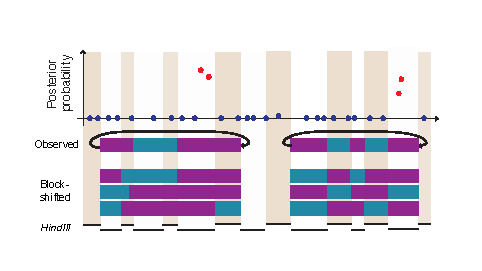
\includegraphics[width=\textwidth]{./figures/blockshifter.pdf}
\caption{Illustration of circularised permutation method for mixed 'superblocks'. Test(Purple) and Control(Turquoise) tissue PIRs are rotated to generate permutations, \textit{Hind}III fragments with no PIRs (grey) are fixed.}
\label{fig:blockshifter}
\centering
\end{figure}

\section{COGS - An algorithm for PCHiC assisted prioritisation of genes and tissues contexts}
We developed an algorithm to compute tissue specific gene scores for each GWAS trait, taking into account linkage disequilibrium, interactions and functional SNP annotation (figure\ref{fig:cogs}). For each gene annotation, for which we have at least one significant interaction and recombination block (used by PMI (see above) to compute trait posterior probabilities)  we compute a block gene score that is composed of three components.

\begin{figure}[h]
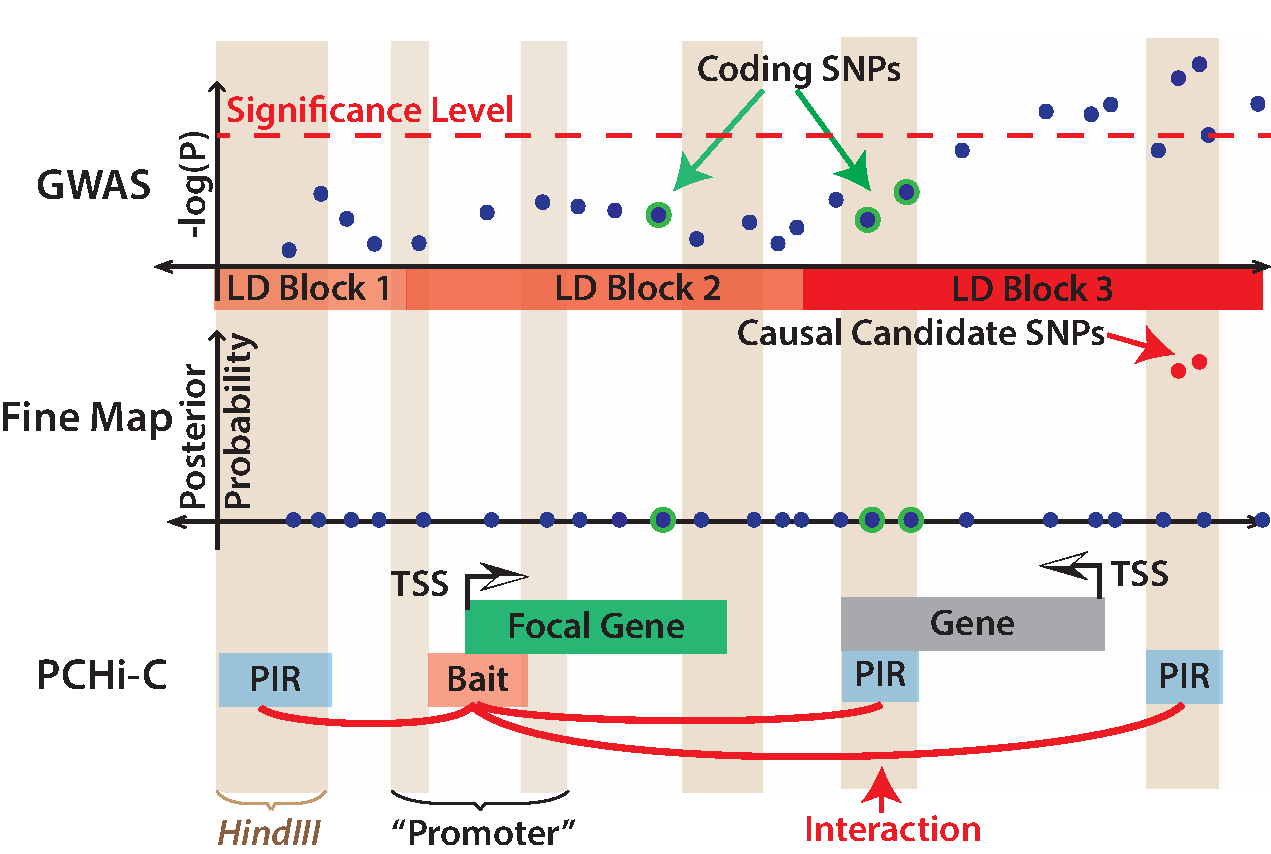
\includegraphics[width=\textwidth]{./figures/cogs3.pdf}
\caption{Illustration of COGS method}
\label{fig:cogs}
\centering
\end{figure}

\begin{enumerate}
\item The contribution due to coding SNPs in the annotated coding gene as computed by VEP .
\item The contribution due to promoter SNPs, which we define as SNPs that overlap a region encompassing the bait and flanking  fragments and not any coding SNPs.
\item The contribution due to SNPs that overlap interacting other ends for a tissue or set of tissues that do not overlap coding SNPs. 
\end{enumerate}

Thus for a given target gene and recombination block we derive a block genescore that is the sum of the posterior probabilities of SNPs overlapping each component.

If we assume independence we can combine blocks to get an overall genescore such that:

\begin{equation}
  Gene\ score = 1- \prod_j  \left(1-\left(\sum_{i \in R_j} 1-PP_i \right) \right)
\end{equation}

Whilst components 1 and 2 are fixed for a given gene and trait the contribution of variants overlapping PIRs varies depending on the tissue context being examined. We developed a hierarchical heuristic method to ascertain for each target gene which was the mostly likely component and cell state. Firstly for each gene we compute the gene score due to genic effects (components 1 $+$ 2) and interactions (component 3) using all available tissue interactions for that gene. We use the ratio of gene effects score to interactions score in a similar manner to a Bayes factor to decide whether one is more likely. If gene effect is more likely (gene.score ratio $>$3) we iterate and compare if the gene score due to coding variants (component 1) is more likely than for promoter variants (component 2). Similarly if an interaction is more likely we compare interaction gene scores for activated vs non-activated cells. If at any stage no branch is substantially preferred over its competitor (ratio of gene scores $<$ 3) we return the previous set as most likely, otherwise we continue until a single cell state/set is chosen. In this way we can prioritize genes based on the overall score and label as to a likely mechanism for candidate causal variants.


%Whilst components 1 and 2 are fixed for a given gene and trait the contribution of SNPs overlapping PIRs varies depending on the tissue context being examined. We developed a hierarchical heuristic method based on the Haematopoietic tree to ascertain for each target gene which was the mostly likely component and tissue context. Firstly for each gene we compute the gene score due to gene effects (components 1 + 2) and interactions (component 3) using all available tissue interactions for that gene. We use the ratio of gene effects score to interactions score in a similar manner to a Bayes factor to decide whether one is more likely. If gene effect is more likely we iterate and compare if the gene score due to coding SNPs (component 1) is more likely than for promoter SNPs (component 2). Similarly if an interaction is more likely we begin descending the Hematopoietic tree and compare interaction gene scores for sets of tissues (e.g Myeloid vs Lymphoid). If at any stage the algorithm is unable to choose it stops and return the previous set as most likely, otherwise it continues until a single tissue/set is chosen. In this way we can prioritize genes based on the overall score and label as to a likely mechanism for candidate causal variants.

\section{COGS gene set enrichment analysis}

To test for enrichment of a gene set for a specific GWAS trait, we used Wilcoxon rank sum tests to compare the distribution of gene prioritisation scores for genes in each HALLMARK set to its complement, within the set of genes that both had membership of at least one HALLMARK set and had a gene score.  We used the $p$ value from this test, together with the difference in mean gene prioritisation scores, to generate a signed $Z$ score, $Z_{ig}$ for trait $i$ and geneset $g$.  To test for relative enrichment in autoimmune diseases versus non-autoimmune traits, we used $t$ tests to compare the distributions of $Z_{ig}$ for $i$ indexing autoimmune diseases to the $Z_{jg}$ for $j$ indexing non-autoimmune traits.


\chapter{Results}

\section{Comparison of PMI with genotype level imputation}

%\subsection{Generation of Promoter Capture Hi-C interaction maps across 17 primary human cell types}
%Promoter Capture Hi-C interaction maps for 17 primary human cell types were generated as part of a collaboration between the Diabetes and Inflammation Laboratory(DIL), Fraser and Spivakov Groups and the BLUEPRINT consortium. Significant interactions were called using CHiCAGO\cite{CairnsFreire-PritchettWingettEtAl2016} (Table\ref{tab:pints}) and these were then reannotated to EnsEMBL 75 using \textit{bedtools}\cite{Quinlan2014}. To enable visual inspection of these results alongside GWAS summary statistics we developed the CHiCP\cite{SchofieldCarverAchuthanEtAl2016} (https://www.chicp.org) webserver. 

%\subsection{Fine mapping of  GWAS summary statistics across 31 traits}
%We created a compendium of GWAS summary statistics from a vareity of sources for 31 traits (Table\ref{tab:gwasm}). In order to maximise resolution and coverage we imputed to 1000 Genome Phase III reference genotype set \cite{1000_Genomes_Project_Consortium2015-wc}. Compare PMI to Imputed. 
%Many studies were missing direction of effect statistics precluding the use of existing summary statistics imputation methods such as  \textit{ImpG}\cite{Pasaniuc2014-im}. We therefore developed an LD based approach, which we named Poor Man's Imputation (PMI).We used Wakefield's\cite{Wakefield2009} synthesis of approximate Bayes factors to compute posterior probabilities for a single variant being causal, within 0.1cM recombination blocks. We masked the MHC region (GRCh37:chr6:25-35Mb) from all downstream analysis due to its extended LD and known strong and complex association with autoimmune diseases.

\section{Tissue specific enrichment of associated variants with PIRs across 31 traits}
We developed a competitive statistical test, \textit{blockshifter}, to examine whether there was evidence for the enrichment of associated variants for tissue specific PIRs across the cell types. \textit{blockshifter}, builds upon the \textit{GOSHIFTER} tool, and uses a circularised permutation technique to account for correlation between (1) neighbouring variants in the GWAS data and (2) neighbouring \textit{Hind}III fragments in the interacting data. Using this method, we found that variants associated with autoimmune disease are enriched at PIRs in lymphoid as compared to myeloid cells.

\section{PCHiC assisted gene prioritisation across 31 traits} 
We next developed COGS, an algorithm to prioritise protein coding genes for each trait. For each gene COGS integrates posterior probabilities for variants overlapping distinct functional categories.
\begin{enumerate}
	\item Protein coding regions.
	\item Gene promoter regions.
	\item PIRs in at least one cell type. 
\end{enumerate}
This enabled us to prioritise 2,604  unique genes (Overall COGS score $>$ 0.5) across all 31 traits examined (table Y). The prioritised genes exhibited enrichments for specific pathways in the Reactome Pathway Database (Fabregat et al., 2016). As expected, genes prioritised for autoimmune diseases were enriched in inflammation and immune response-related pathways, such as interleukin and T cell receptor signaling, whereas genes prioritised for platelet traits were preferentially associated with platelet production and hemostasis (Figure X). 

%\section{Context specific gene priortisation across activated CD4$^{+}$ activated T cells}
\section{Fine mapping and gene prioritisation acriss 8 densely genotyped autoimmune diseases}
Focussing on autoimmne traits we added additional summary statistics for xx diseases genotyped on the ImmunoChip platform. We computed posterior probabilities in a similar fashion replacing 0.1cM blocks for 187 regions that were targetd for dense genotyping on this platform. For four traits we had access genotype level data and we used GUESSFM to compute multi-SNP causal variant models which were used to compute marginal posterior probabilities. We focused our attention to activated and non activated CD4$^{+}$ promoter interaction maps and extended COGs to incorporate a simple binary decision tree model to allow tissue or functional category resolution.  Across the combined GWAS and ImmunoChip datasets we were able prioritise xx genes (figure tree), which was reduced to xx on further filtering using gene expression data and overlap with known disease susceptibility regions as curated by ImmunoBase.

\section{Promoter contacts underlie context specific allelic expression of \textit{IL2RA}}
Using COGS \textit{IL2RA} was prioritised in multiple diseases (what are they ?), we found this prioritisation to be driven by an interaction between the IL2RA promoter and a PIR in exon 1 known to harbour a set of type 1 diabetes putative causal SNPs (figure z) indentified in a previous fine mapping study\cite{WallaceCutlerPontikosEtAl2015}. This set of SNPs is in high LD with 495 which has been shown to affect the surface expression CD25 in naive memory T cells\cite{DendrouPlagnolFungEtAl2009}. We adapted a method previously used to perform targetted bisulphite sequencing to examine 660 for evidence of alleleic expression. We observed allelic imbalance  in non activated CD4$^{+}$ T cells however on activation this was lost suggesting a context specific effect within this locus.

\chapter{Discussion and Future Work}
\section{CHiCP - A platform for visual integration and results disemination}
\section{blockshifter and COGS refinement}
\subsection{Assuumption examination}
\subsection{Stand alone code development}
\subsection{Data driven approach to understanding COGS scores}
% Can we use Mary's ABC approach to generate GWAS with known causal variants and see how this affects COGS scores.
\subsection{Integration of functional data through data driven variable priors}
%FGWAS but also rare autoimmune phenotypes - need to discuss masking - see https://genomestake.blogspot.co.uk/2016/06/thirtieth-take-resilience-and.html for an interesting discussion of expressivity and penetrance.
\section{PCHiC eQTL and GWAS colocalisation}
\section{Development of methods for tissue specific gene set enrichment analysis}
\section{PCHiC modelling of local gene networks} 
\chapter{Appendix}

	%\begin{savenotes}
{\begin{table}[ht]
\caption{Summary of PCHi-C datasets used in this study. Adapted from Javierre et al. (Under review)}
\centering
%\begin{tabularx}{\linewidth}{l l r l l }
%\begin{tabularx}{\linewidth}{X l r l l }
{\tabulinesep=1.2mm
\begin{tabular}{| L{3cm} | C{2cm} | C{2cm} | C{2.6cm} | C{2cm} | }
  \hline
 \rowcolor{white}
 Cell type & Acronym & Biological replicates & Unique captured read pairs & Detected interactions \\
  \hline
 Megakaryocytes & MK &   4 & 653,848,788 & 150,203 \\
 Erythroblasts & Ery &   3 & 588,786,672 & 144,771 \\
 Neutrophils & Neu &   3 & 736,055,569 & 131,609 \\
 Monocytes & Mon &   3 & 572,357,387 & 151,389 \\
 Macrophages M0 & M$\phi0$ &   3 & 668,675,248 & 163,791 \\
 Macrophages M1 & M$\phi1$ &   3 & 497,683,496 & 163,399 \\
 Macrophages M2 & M$\phi2$ &   3 & 523,561,551 & 173,449 \\
 Endothelial Precursors & EndP &   3 & 420,536,621 & 141,382 \\
 Naive B cells & nB &   3 & 629,928,642 & 171,439 \\
 Total B cells & tB &   3 & 702,533,922 & 183,119 \\
 Fetal Thymus & FetT &   3 & 776,491,344 & 145,577 \\
 Naive CD4+ T cells & nCD4 &   4 & 844,697,853 & 192,048 \\
 Total CD4+ T cells & tCD4 &   3 & 836,974,777 & 166,668 \\
 Non-Activated Total CD4+ T cells & naCD4 &   3 & 721,030,702 & 177,371 \\
 Activated Total CD4+ T cells & aCD4 &   3 & 749,720,649 & 188,714 \\
 Naive CD8+ T cells & nCD8 &   3 & 747,834,572 & 187,399 \\
 Total CD8+ T cells & tCD8 &   3 & 628,771,947 & 183,964 \\
 \hline
 \hline
 \rowcolor{gray!50}
 Total & & & 11,299,489,740 & 708,007\tablefootnote{Unique interactions captured in at least one cell type} \\
 \hline
\end{tabular}}
\label{tab:pints}
\end{table}
\addtocounter{footnote}{+1}
}
%\end{savenotes}
	\begin{landscape}
	 	
%\begin{table}[ht]
\begin{center}

\centering
\begin{longtable}{| L{5cm} | C{1.2cm} | C{1cm} | C{1.5cm} | C{1.5cm} | C{1.5cm} | L{2.5cm} | R{1.5cm} | L{4cm} |}
\caption{Summary of GWAS summary statistics used in this study}\label{tab:gwasm}\\
  \hline\rowcolor{white}   Trait & Acronym & Cases & Controls & Study Type & PMID & First Author(Date) & \# SNPs  & Source \\ \hline \hline  
  \endfirsthead
  \hline  \rowcolor{white} Trait & Acronym & Cases & Controls & Study Type & PMID & First Author(Date) & \# SNPs  & Source \\ \hline \hline 
  \endhead
  \hline \rowcolor{white} \multicolumn{9}{|r|}{{Continued on next page}} \\ \hline 
  \endfoot
  \rowcolor{white}\hline \hline 
  \endlastfoot

Platelet volume & PV & 18600 &  & QUANT & 22139419 & Gieger(2011) & 2231438  & N Soranzo personal communication \\
Platelet count & PLT & 48666 &  & QUANT & 22139419 & Gieger(2011) & 2206665  & N Soranzo personal communication \\
Mean corpuscular volume & MCV & 4627 &  & QUANT & 19820697 & Soranzo(2009) & 2156669  & N Soranzo personal communication \\
Packed cell volume & PCV & 4627 &  & QUANT & 19820697 & Soranzo(2009) & 2009357  & N Soranzo personal communication \\
Red blood cell count & RBC & 4627 &  & QUANT & 19820697 & Soranzo(2009) & 2091590  & N Soranzo personal communication \\
Haemoglobin & HB & 4627 &  & QUANT & 19820697 & Soranzo(2009) & 1640923  & N Soranzo personal communication \\
Mean corpuscular haemoglobin & MCH & 4627 &  & QUANT & 19820697 & Soranzo(2009) & 1904974  & N Soranzo personal communication \\
Mean corpuscular haemoglobin concentration & MCHC & 4627 &  & QUANT & 19820697 & Soranzo(2009) & 2070334  & N Soranzo personal communication \\
Ulcerative colitis Anderson & UC & 6687 & 19718 & CC & 21297633 & Anderson(2011) & 1399283  & \url{http://www.immunobase.org} \\
Multiple sclerosis IMSGC & MS & 9772 & 17376 & CC & 21833088 & IMSGC(2011) & 463628  & \url{http://www.immunobase.org} \\
Type 1 diabetes Barrett & T1D & 8000 & 8000 & CC & 19430480 & Barrett(2009) & 789849  & \url{http://www.immunobase.org} \\
Celiac disease DuBois & CEL & 4533 & 10750 & CC & 20190752 & Dubois(2010) & 509768  & \url{http://www.immunobase.org} \\
Crohn's disease immunobase & CD & 6333 & 15056 & CC & 21102463 & Franke(2010) & 950208  & \url{http://www.immunobase.org} \\
Rheumatoid arthritis Okada & RA & 14361 & 43923 & CC & 24390342 & Okada(2014) & 8513749  & \url{http://plaza.umin.ac.jp/\~okada/datasource/files/GWASMetaResults/RA\_GWASmeta\_European\_v2.txt.gz} \\
Type 2 diabetes & T2D & 12171 & 56860 & CC & 22885922 & Morris(2012) & 2075585  & \url{http://diagram-consortium.org/downloads.html} \\
Height & HT & 253288 &  & QUANT & 25282103 & Wood(2014) & 1927160  & \url{https://www.broadinstitute.org/collaboration/giant/images/0/01/GIANT\_HEIGHT\_Wood\_et\_al\_2014\_publicrelease\_HapMapCeuFreq.txt.gz} \\
Tryglycerides & TG & 96598 &  & QUANT & 20686565 & Teslovich(2010) & 2304026  & \url{http://csg.sph.umich.edu/abecasis/public/lipids2010/TG2010.zip} \\
High density lipoprotein & HDL & 99900 &  & QUANT & 20686565 & Teslovich(2010) & 2322449  & \url{http://csg.sph.umich.edu/abecasis/public/lipids2010/HDL2010.zip} \\
Low density lipoprotein & LDL & 95454 &  & QUANT & 20686565 & Teslovich(2010) & 2298548  & \url{http://csg.sph.umich.edu/abecasis/public/lipids2010/LDL2010.zip} \\
Total Cholesterol & TC & 100184 &  & QUANT & 20686565 & Teslovich(2010) & 2323152  & \url{http://csg.sph.umich.edu/abecasis/public/lipids2010/TC2010.zip} \\
Glucose sensitivity BMI adjusted & GLC\_B & 58074 &  & QUANT & 22581228 & Manning(2012) & 2622994  & \url{ftp://ftp.sanger.ac.uk/pub/magic/MAGIC\_Manning\_et\_al\_FastingGlucose\_MainEffect.txt.gz} \\
Glucose sensitivity & GLC & 58074 &  & QUANT & 22581228 & Manning(2012) & 2622996  & \url{ftp://ftp.sanger.ac.uk/pub/magic/MAGIC\_Manning\_et\_al\_FastingGlucose\_MainEffect.txt.gz} \\
Insulin sensitivity BMI adjusted & INS\_B & 51750 &  & QUANT & 22581228 & Manning(2012) & 2621974  & \url{ftp://ftp.sanger.ac.uk/pub/magic/MAGIC\_Manning\_et\_al\_lnFastingInsulin\_MainEffect.txt.gz} \\
Insulin sensitivity & INS & 51750 &  & QUANT & 22581228 & Manning(2012) & 2621977  & \url{ftp://ftp.sanger.ac.uk/pub/magic/MAGIC\_Manning\_et\_al\_lnFastingInsulin\_MainEffect.txt.gz} \\
Femoral neck bone mineral density & FNBMD & 32961 &  & QUANT & 22504420 & Estrada(2012) & 2473840  & \url{http://www.gefos.org/sites/default/files/GEFOS2\_FNBMD\_POOLED\_GC.txt.gz} \\
Lumbar spine bone mineral density & LSBMD & 32961 &  & QUANT & 22504420 & Estrada(2012) & 2463611  & \url{http://www.gefos.org/sites/default/files/GEFOS2\_LSBMD\_POOLED\_GC.txt.gz} \\
Diastolic blood pressure & BP\_D & 69395 &  & QUANT & 21909115 & ICBP(2011) & 2460847  & \url{http://www.georgehretlab.org/ICBP-summary-Nature.csv.gz} \\
Systolic blood pressure & BP\_S & 69395 &  & QUANT & 21909115 & ICBP(2011) & 2460847  & \url{http://www.georgehretlab.org/ICBP-summary-Nature.csv.gz} \\
Body Mass Index & BMI & 322200 &  & QUANT & 25673413 & Locke(2015) & 1984096  & \url{https://www.broadinstitute.org/collaboration/giant/images/1/15/SNP\_gwas\_mc\_merge\_nogc.tbl.uniq.gz} \\
Systemic Lupus Erythrematosis & SLE & 4036 & 6959 & CC & 26502338 & Bentham(2015) & 7734064  & \url{http://www.immunobase.org} \\
Primary Billiary Cirrhosis & PBC & 2764 & 10475 & CC & 26394269 & Cordell(2015) & 1134133  & \url{http://www.immunobase.org} \\
  
\end{longtable}
\end{center}
%\end{table}
	\end{landscape}

\bibliographystyle{plain}
\bibliography{first_year_report}

\end{document}